\chapter{Comprehensive Multi-Root Planning}

ABSTRACT:
We formulate and study the
\emph{comprehensive multi-root} (CMR) planning problem,
in which feasible paths are desired between multiple regions.
We propose two primary contributions which allow us to extend
state-of-the-art sampling-based planners.
First, we propose the notion of \emph{vertex coloring} as a compact
representation of the CMR objective on graphs.
Second, we propose a method for \emph{deferring edge evaluations}
which do not advance our objective, by way of a simple
criterion over these vertex colorings.
The resulting approach can be applied to any CMR-agnostic 
graph-based planner which evaluates a sequence of edges.
We prove that the theoretical performance of the colored algorithm
is always strictly better than (or equal to)
that of the corresponding uncolored version.
We then apply the approach to the Probabalistic RoadMap (PRM)
algorithm;
the resulting \emph{Colored Probabalistic RoadMap} (cPRM)
is illustrated on 2D and 7D CMR problems.

\section{Introduction}
\label{sec:intro}

Many real-world tasks require a robot to quickly accomplish multiple
subtasks without a prescribed order.
Consider a personal assistant robot
clearing several objects from a tabletop,
or a manufacturing robot performing several welds on a novel workpiece.
Furthermore,
each subtask often permits multiple suitable robot configurations such as
grasps of an object or orientations of a tool.
Even if only one end effector pose is valid,
manipulator redundancy enables many feasible configurations. 
We are interested in efficiently finding feasible paths
for such problems.

For example, consider the robot in Figure~\ref{subfig:herb-picture}.
It is tasked with using a handheld drill to tighten three bolts (blue)
during assembly of a truss structure.
Each bolt permits an entire manifold of permissible robot
configurations which would allow completion of the sub-task,
many of which may be either directly infeasible or difficult to reach
given the environment and other subtasks. We call each of these configurations 
a \emph{root}, and collect all roots which satisfy a particular subtask
into a \emph{root set}. 

The planning problem, then,
can be formulated as finding a diverse set of paths between these
root sets.
We formalize this problem as the \emph{comprehensive multi-root} (CMR)
planning problem (Section~\ref{sec:def}) and ask the question: 
\begin{quote}
How can we efficiently maximize connections between pairs of roots
in \emph{different} root sets?
\end{quote}
Figure~\ref{subfig:cmr-illustration} illustrates a partial solution
to a problem with three root sets where $6$
out of a total possible $27$ connections have been discovered.

\begin{figure}[t]
\centering
\begin{subfigure}[b]{0.6\linewidth}
\centering
\includegraphics[width=\linewidth]{figs/herb-drilling.png}
\caption{A real-world problem.}
\label{subfig:herb-picture}
\end{subfigure}
%\\ \quad \\
\begin{subfigure}[b]{0.35\linewidth}
\centering
\resizebox{\linewidth}{!}{
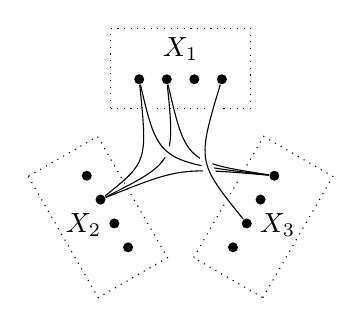
\begin{tikzpicture}[scale=0.7]

\begin{scope}
\node[rectangle,draw,dotted,
   inner sep=0,minimum height=0.4in,minimum width=0.7in] (x1) at (0,0) {};
\node[below] at (x1.north) {$X_1$};
\node[circle,inner sep=0,minimum size=0.05in,fill=black] (x1a) at (-0.75,-0.2) {};
\node[circle,inner sep=0,minimum size=0.05in,fill=black] (x1b) at (-0.25,-0.2) {};
\node[circle,inner sep=0,minimum size=0.05in,fill=black] (x1c) at ( 0.25,-0.2) {};
\node[circle,inner sep=0,minimum size=0.05in,fill=black] (x1d) at ( 0.75,-0.2) {};
\end{scope}

\begin{scope}[shift={(-1.5,-2.7)},rotate=120]
\node[rectangle,draw,dotted,rotate=120,
   inner sep=0,minimum height=0.4in,minimum width=0.7in] (x2) at (0,0) {};
\node at (0,0.3) {$X_2$};
\node[circle,inner sep=0,minimum size=0.05in,fill=black] (x2a) at (-0.75,-0.2) {};
\node[circle,inner sep=0,minimum size=0.05in,fill=black] (x2b) at (-0.25,-0.2) {};
\node[circle,inner sep=0,minimum size=0.05in,fill=black] (x2c) at ( 0.25,-0.2) {};
\node[circle,inner sep=0,minimum size=0.05in,fill=black] (x2d) at ( 0.75,-0.2) {};
\end{scope}

\begin{scope}[shift={(1.5,-2.7)},rotate=-120]
\node[rectangle,draw,dotted,rotate=-120,
   inner sep=0,minimum height=0.4in,minimum width=0.7in] (x3) at (0,0) {};
\node at (0,0.3) {$X_3$};
\node[circle,inner sep=0,minimum size=0.05in,fill=black] (x3a) at (-0.75,-0.2) {};
\node[circle,inner sep=0,minimum size=0.05in,fill=black] (x3b) at (-0.25,-0.2) {};
\node[circle,inner sep=0,minimum size=0.05in,fill=black] (x3c) at ( 0.25,-0.2) {};
\node[circle,inner sep=0,minimum size=0.05in,fill=black] (x3d) at ( 0.75,-0.2) {};
\end{scope}

\draw (x1b) .. controls(-0.1,-1.7) .. (x2c);
\draw[white,line width=4] (x1a) .. controls(-0.4,-1.7) .. (x3a);
\draw (x1a) .. controls(-0.4,-1.7) .. (x3a);
\draw (x1b) .. controls( 0.1,-1.7) .. (x3a);
\draw (x1a) .. controls(-0.6,-1.7) .. (x2c);
\draw (x3a) .. controls(0.0,-1.8) .. (x2c);
\draw[white,line width=4] (x1d) .. controls( 0.3,-1.7) .. (x3c);
\draw (x1d) .. controls( 0.3,-1.7) .. (x3c);

\end{tikzpicture}
}
\caption{Illustration.}
\label{subfig:cmr-illustration}
\end{subfigure}
\caption{The comprehensive multi-root (CMR) problem.}
\label{fig:cmr-problems}
\end{figure}

\begin{figure*}[t]
\centering
\begin{minipage}{.49\textwidth}
\begin{subfigure}[b]{.49\linewidth}
\centering
\includegraphics{build/w13-fu1-ec86}
\caption{PRM (86 Edges Checked)\\(195 Edges Considered, No Pairs)}
\label{subfig:w13-sameec-uncolored}
\end{subfigure}
\begin{subfigure}[b]{.49\linewidth}
\centering
\includegraphics{build/w13-fs1-ec86}
\caption{cPRM (86 Edges Checked)\\(344 Edges Considered, 1 Pair)}
\label{subfig:w13-sameec-colored}
\end{subfigure}
\\ \quad \\
\begin{subfigure}[b]{.49\linewidth}
\centering
\includegraphics{build/w13-fu1-ei344}
\caption{PRM (344 Edges Considered)\\(125 Edges Checked, 8 Pairs)}
\label{subfig:w13-sameein-uncolored}
\end{subfigure}
\begin{subfigure}[b]{.49\linewidth}
\centering
\includegraphics{build/w13-fs1-ei344}
\caption{cPRM (344 Edges Considered)\\(91 Edges Checked, 8 Pairs)}
\label{subfig:w13-sameein-colored}
\end{subfigure}
\end{minipage}
\begin{minipage}{.49\textwidth}
\begin{subfigure}[b]{\linewidth}
\centering
\includegraphics{build/plot-edges-w13}
\caption{Edges considered, evaluated, deferred, and skipped.}
\label{subfig:w13-plot-edges}
\end{subfigure}
\\ \quad \\
\begin{subfigure}[b]{\linewidth}
\centering
\begin{tikzpicture}[font=\scriptsize]
% primary axis
\begin{axis}[
   xlabel={Edges Checked},
   ylabel={Pairs Connected},
   %legend pos= north west,
   legend style={at={(axis cs:5,7.5)},anchor=north west},
   legend cell align=left,
   %axis equal image,
   width=\columnwidth,
   height=1.3in,
   xmin=0, xmax=150,
   %xmin=0, xmax=1000, ymin=0,
   %scaled ticks=base 10:-3,
   xlabel near ticks,
   ylabel near ticks]
\addplot[black,ultra thick] table[col sep=space] {figs/w13-fu1-qs-pvc.txt};
\addlegendentry{Uncolored}
\addplot[mark=*,black,only marks,mark size=1,forget plot] plot coordinates {
   (125,8) % uc
};
\addplot[green,thick] table[col sep=space] {figs/w13-fs1-qs-pvc.txt};
\addlegendentry{Colored}
\addplot[mark=*,black,only marks,mark size=1,forget plot] plot coordinates {
   (86,1) %+1
   (87,2) %+1
   (89,4) %+2
   (90,6) %+2
   (91,8) %+2
};
\addplot[blue,mark=o,mark size=2] plot coordinates {(86,0) (86,1)}; % a-b comparison
\addplot[blue,mark=o,mark size=2] plot coordinates {(125,8) (91,8)}; % c-d comparison
% coordinates
\coordinate (subfig_a_point) at (axis cs: 86,0);
\coordinate (subfig_b_point) at (axis cs: 86,1);
\coordinate (subfig_c_point) at (axis cs: 125,8);
\coordinate (subfig_d_point) at (axis cs: 91,8);
\end{axis}
% labels
\node[circle,inner sep=0pt,color=blue,fill=white] (subfig_b_label) at (2.9,0.6) {(b)};
\node[circle,inner sep=0pt,color=blue,fill=white] (subfig_d_label) at (3.1,1.3) {(d)};
\node[circle,inner sep=0pt,color=blue,fill=white] (subfig_a_label) at (4.9,0.5) {(a)};
\node[circle,inner sep=0pt,color=blue,fill=white] (subfig_c_label) at (5.2,1.2) {(c)};
\draw[color=blue,->] (subfig_b_label) -- ($ (subfig_b_point)!4pt!(subfig_b_label) $);
\draw[color=blue,->] (subfig_d_label) -- ($ (subfig_d_point)!4pt!(subfig_d_label) $);
\draw[color=blue,->] (subfig_a_label) -- ($ (subfig_a_point)!4pt!(subfig_a_label) $);
\draw[color=blue,->] (subfig_c_label) -- ($ (subfig_c_point)!4pt!(subfig_c_label) $);
\end{tikzpicture}
\caption{CMR Objective vs edges evaluted.}
\label{subfig:w13-plot-pairs}
\end{subfigure}
\end{minipage}
\caption{A comparison between an
   uncolored~(\ref{subfig:w13-sameec-uncolored},\ref{subfig:w13-sameein-uncolored})
   and colored~(\ref{subfig:w13-sameec-colored},\ref{subfig:w13-sameein-colored})
   forest-of-trees PRM on the same sequence of edges.
   Plot~(\ref{subfig:w13-plot-edges}) shows the evolution of edges in both
   algorithms as they progress,
   and plot~(\ref{subfig:w13-plot-pairs}) shows the number of between-rootset
   pairs found by each.}
\label{fig:example-w13-figstar}
\end{figure*}

We focus our attention on graph-based planners
(e.g. the PRM \cite{kavrakietal1996prm}) 
which build an \emph{explicit} graph approximating the free
configuration space of the robot by incrementally evaluating (for collisions) 
an \emph{implicit} graph comprising edges between sampled vertices
(Section~\ref{sec:cmr-graphs}).
This explicit graph is then queried to find feasible paths between
different roots.

We can abstract these algorithms as edge sources which are emitting
potential edges for evaluation.
Our key insight is to introduce a \emph{deferred edge queue} 
which postpones the evaluation of certain edges in order to
maximize the CMR objective during planning.

We do so by formally representing the CMR objective
in terms of \emph{vertex coloring}.
This naturally suggests an evaluation criterion which we can use to
prioritize some edge evaluations over others (Section~\ref{sec:gen-sol}).
When applied to any edge-evaluating algorithm,
the resulting colored algorithm is provably superior to the original
(Section~\ref{sec:analysis}).

As an example of this approach,
we implemented a colored version of the PRM algorithm
(Section~\ref{sec:colored-prm}),
and applied it to CMR problems in 2D and 7D.

Figure~\ref{fig:example-w13-figstar} shows the results of running
both the uncolored and colored versions of the forest-of-trees PRM
on a 2D problem with two root sets (one at top, one at bottom).
Each algorithm works on the same set of samples;
since they share the same connection rule,
this induces the same set of potential edges.
The remainder of this section calls out the primary features of colored
algorithms by way of this example.

Fig.~\ref{subfig:w13-sameec-uncolored}
and~\ref{subfig:w13-sameec-colored}
compare the tree states of the algorithms
after having performed a collision check on the same number of edges (86).
Bolded edges show the difference between the free-edge
graphs built by each algorithm.
By this point, the colored algorithm has found its first connection between
the two root sets (at right, shown in violet),
whereas the uncolored algorithm has yet to find a connection.
This is possible because the colored algorithm has chosen to defer
evaluation of many edges (shown in light grey).

Fig.~\ref{subfig:w13-sameein-uncolored}
and~\ref{subfig:w13-sameein-colored}
show a different comparison.
In this case,
the tree states are compared after each algorithm has finished considering
the same number of edges (344).
Here, both algorithms have achieved the same objective by
connecting the same number of pairs (8).
However, the tree built by the colored algorithm is a subset of that
built by the uncolored one;
it has therefore performed fewer edge evaluations (91 to 125).

Figure~\ref{subfig:w13-plot-edges} shows the evolution of edges
for each algorithm.
When the uncolored algorithm considers each edge,
it is either checked for collision (below the black line)
or skipped in order to maintain a forest of trees (above the black line).
The colored algorithm additionally maintains a queue of deferred edges
(pattern).
This allows it to perform fewer edge evaluations (below the green line)
for a given input edge.
In Section~\ref{sec:analysis}, we prove that these deferments
do not affect the CMR objective.
The tree state comparisons discussed above are called out in blue.
Each edge evaluation which results in additional connected pairs is
additionally denoted with a black circle.

Figure~\ref{subfig:w13-plot-pairs} shows the number of connected inter-root
pairs as a function of the number of edges evaluated.
The colored algorithm finds its first pair earlier than the uncolored
algorithm (86 vs 125).
Once the colored algorithm finds one pair,
it quickly finds others.
Again, the tree state comparisons are called out in blue.

\section{Related Work}
\label{sec:related}

While our formulation of the CMR problem itself is newly introduced,
so that no existing planners are explicitly tailored for it,
it is intimately related to several classes of well-studied
motion planning problems.

The classical FindPath or mover's problem
\cite{choset2005robotmotion}, \cite{lavalle2006planningbook}
concerns finding a path between two single states.
However,
many approaches are designed to handle connections
between multiple starts, goals, or both.
A problem with multiple starts and goals can be represented as a CMR problem
with $N=2$ root sets.

For example, the original A* algorithm \cite{hart1968astar}
searched for a path between a single start state
and multiple goal states.
While single-query sampling-based algorithms such as the RRT
\cite{lavallekuffner1999rrt}, \cite{kuffner2000rrtconnect}
generally consider a single start and goal state,
extensions \cite{berenson2009manifolds}
have allowed such planners to consider both multiple starts and multiple
goals.
Trajectory optimization can also be applied to the motion planning problem;
while typically considered for single start and goal states,
recent generalizations \cite{dragan2011goalsets}, \cite{schulman2013trajopt}
have extended them to sets of starts or goals.

However, even those approaches that handle start and/or goal sets
typically terminate once a single path is found,
and do not attempt to find multiple diverse connections
between different root sets.

To accomodate more than two root sets,
approaches for multi-query planning
(e.g. \cite{kavrakietal1996prm}) may appear better suited for finding
multiple diverse connections.
For example, they have been used for efficiently solving the single-object
manipulation problem \cite{simeon2004manipulation}.

Additionally, some approaches perform similar deferment on edge
evaluations to our approach.
For example, so-called ``lazy'' algorithms,
such as \cite{bohlin2000lazyprm}, \cite{sanchezante2001sbl}
defer collision checking until edges are to be used.

Other recent work has married symbolic reasoning with geometric planning
for tasks with multiple subtasks
as multi-modal planning \cite{hauser2010multi},
temporal logic \cite{bhatia2010temporalgoals},
or hierarchical or bridged representations and interfaces
\cite{cambon2009hybrid}, \cite{gravot2005asymov},
\cite{srivastava2014taskmotion}.

\section{The Comprehensive Multi-Root Problem}
\label{sec:def}

We work with the robot's configuration space $X$
and its collision-free subset $X_{free}$.
We consider the general problem with $N$ root sets in this space
$\{ X_1, \dots, X_N \}$.
We seek a diverse set of feasible paths between root sets
-- that is, we want to maximize the number of connected roots between sets. 
We call this the \emph{comprehensive multi-root} (CMR) planning problem.

We track progress via the $r$-score:
\begin{equation}
   r = \big| \{
      \textsc{Path}(x_a,x_b) \;|\; x_a,x_b~\text{in different root sets}
      \} \big|.
   \label{eqn:obj}
\end{equation}
For example, the solution illustrated in Figure~\ref{subfig:cmr-illustration}
has an $r$-score of 6 out of a maximum of 27.
Our objective is to \emph{maximize} the $r$-score as \emph{quickly} as
possible.
We define this more formally next.

\section{The CMR Problem on Graphs}
\label{sec:cmr-graphs}

\begin{algorithm}[t]
\caption{Edge Evaluation (graph or forest)}
\begin{algorithmic}[1]
%\Procedure{EvaluateGraph}{$g, v_a, v_b$}
%\If {$\mbox{\textsc{EdgeFree}}(v_a, v_b)$}
%\State $g.E \leftarrow g.E \cup \{ (v_{a}, v_{b}) \}$
%\EndIf
%\EndProcedure
\Procedure{Evaluate}{$g, v_a, v_b$}
\If {$v_a$ and $v_b$ in same connected component}
\State \Return \Comment{Optional, for forest}
\EndIf
\If {$\mbox{\textsc{EdgeFree}}(v_a, v_b)$}
\State $g.E \leftarrow g.E \cup \{ (v_{a}, v_{b}) \}$
\EndIf
\EndProcedure
\end{algorithmic}
\label{alg:edge-evaluators}
\end{algorithm}

We focus on motion planning approaches where
$X_{free}$ is approximated by a graph $g$.
For example,
in a search-based planning approach such as A$^*$ \cite{hart1968astar},
$g$ is a state-lattice,
whereas in a sampling-based planning approach such as the
PRM \cite{kavrakietal1996prm},
$g$ is a random geometric graph.

A key feature of these approaches is that the graph $g$ is \emph{implicit},
i.e. incrementally discovered and/or evaluated as the search progresses.
For example, in a PRM, a sample is drawn at random from $X_{free}$,
all of the local paths to its neighbors on $g$
are evaluated for collisions (using a function
like Algorithm~\ref{alg:edge-evaluators})
and collision-free paths are incrementally added to $g$ as edges.

However, for applications we're interested in,
edge evaluations are expensive \cite{lavalle2006planningbook}
because they require several collision checking queries between
complex geometries.
We therefore want to maximize our objective \eqref{eqn:obj}
while minimizing the number of edges to be checked.
To accomplish this, we return to our CMR objective.

\section{A General Technique for Fast CMR Planning on Graphs}
\label{sec:gen-sol}

We use the structure of the CMR problem
to motivate a new class of algorithms.
We do so by redefining our objective in terms of the graph's structure,
and then describing the two insights which characterize our approach:
\emph{coloring vertices} and \emph{deferring edges}.
We then show how an algorithm can be extended to include these features.

\subsection{Viewing our Objective with Vertex and Graph Colorings}

Consider a graph $g$ in $X_{free}$
applied to a CMR problem.
Here, we show how we can succinctly represent our objective
(\ref{eqn:obj}) with respect to this graph.

We define the \emph{coloring} ${\bf c}(v)$ of vertex $v$ as
\begin{equation}
   \arraycolsep=1.4pt
   %{\bf c}(v) = [c_1, \dots c_N]^\top
   {\bf c}(v) = \hspace{-0.03in} \left[\begin{array}{c}
   c_1 \\ \vdots \\ c_N \\
   \end{array}\right]
   \mbox{ with }
   c_i = \big| \{
      \textsc{Path}(v,x) \;|\; x \in X_i
      \} \big|.
\end{equation}
The coloring\footnote{
Our use of the term ``coloring'' with respect to graph vertices
is not to be confused with the proper graph color assignment problem.}
of a vertex is an $N$-vector,
with each element $c_i$ the number of reachable roots
in the corresponding root set $X_i$ w.r.t. the graph.

Further, we define the \emph{colored norm} $||\cdot||$ as
\begin{equation}
   ||{\bf c}(v)|| = \sum c_i c_j \mbox{ for } i < j.
\end{equation}
The colored norm counts the number of pairs of roots in different root sets
that are connected through the vertex. 

\begin{proposition}
Every vertex in a given connected component $k$ has the same coloring
${\bf c}_k$.
\end{proposition}
\begin{proof}
By definition, every vertex in a connected component has a
\textsc{Path} to every other vertex;
therefore the color of all constituent vertices is equal.
\end{proof}

We now define the colored norm of a connected component as the colored norm
of \emph{any} of its constituent vertices.

Finally, we define the colored norm of a graph $g$
as the sum of the colored norms of all of its connected components:
\begin{equation}
   \label{eqn:colored-norm-graph}
   ||g|| = \sum_k ||{\bf c}_k||
\end{equation}
For a graph solving a CMR problem,
the colored norm of the graph (\ref{eqn:colored-norm-graph})
is equal to the CMR objective (\ref{eqn:obj}).
%\cdnote{Do I need to show this?}

\subsection{Prioritizing Edges via the Graph's Colored Norm}

Due to the expense of evaluating edges
as mentioned in Section~\ref{sec:cmr-graphs},
we endeavor to maximize the CMR objective
(\ref{eqn:colored-norm-graph})
while minimizing the number of edges evaluated.
The reformulation of the objective in terms of graph and vertex coloring
suggests a method to prioritize certain edge evaluations over others.

We first consider the myopic criterion
shown in Algorithm~\ref{alg:criterion}.
When a potential edge between two vertices $v_a,v_b$ is considered,
we determine whether the inclusion of this edge in our graph $g$
would immediately improve our objective.
If so, we proceed to evaluate the edge.

\begin{algorithm}[t!]
\begin{algorithmic}[1]
\Function{MyopicCriterion}{$g, v_a, v_b$}
\State $g'.V \leftarrow g.V$
\State $g'.E \leftarrow g.E \cup \{(v_a, v_b)\}$
\If {$||g'|| > ||g||$}
   \Comment{Check objective}
\State \Return True
   \Comment{Evaluate edge}
\Else
\State \Return False
   \Comment{Do not evaluate edge}
\EndIf
\EndFunction
\Function{Criterion}{$g, v_a, v_b$}%
   \Comment{Balanaced}%
\State $g'.V \leftarrow g.V$
\State $g'.E \leftarrow g.E \cup \{(v_a, v_b)\}$
\If {$||g'|| > ||g||$}
   \Comment{Check objective}
\State \Return True
   \Comment{Evaluate edge}
\ElsIf {exatly one of ${\bf c}(v_a),{\bf c}(v_b)$ is ${\bf 0}$}
\State \Return True
   \Comment{Evaluate edge}
\Else
\State \Return False
   \Comment{Do not evaluate edge}
\EndIf
\EndFunction
\end{algorithmic}
\caption{Myopic and Balanced Edge Criterions}
\label{alg:criterion}
\end{algorithm}

Unfortunately, when initialized with a graph consisting of only
roots,
this criterion will only allow edges which connect directly
between roots of different root sets.
In complex problems, the probability that such edges are feasible
is quite low --
the purpose of intermediate vertices is to find a path within
complex $X_{free}$ spaces.

Therefore, we propose a balanced criterion which allows for exploration
of $X_{free}$.
This approach additionally evaluates edges which would provide an
uncolored vertex (i.e. with ${\bf c}(v) = {\bf 0}$) an initial coloring.

\subsection{A Compact Depiction of Vertex Coloring}

Note that in the graph colored norm test
$||g'|| > ||g||$,
the new graph $g'$ differs from $g$ by a single new edge $(v_a,v_b)$.
In the case that $v_a$ and $v_b$ are already in the same connected component,
the additional edge trivially has no effect on the colored norm,
and the test fails.
Otherwise, the test can be restated as
\begin{equation}
   ||g'|| > ||g||
   \mbox{~iff~}
   ||{\bf c}_a+{\bf c}_b|| > ||{\bf c}_a|| + ||{\bf c}_b||.
\end{equation}
By definition of the colored norm,
taking for brevity ${\bf c}_x = [x_1,\dots,x_N]^\top$,
we can restate the inequality as
\begin{equation}
   \sum_{i<j} (a_i+b_i)(a_j+b_j) > \sum_{i<j} a_i a_j + \sum_{i<j} b_i b_j
\end{equation}
\begin{equation}
   \sum_{i<j} a_i b_j + \sum_{i<j} b_i a_j > 0
\end{equation}
or simply
\begin{equation}
   ||g'|| > ||g||
   \mbox{~iff~}
   a_i,b_j
   \mbox{~nonzero for some~} i \neq j.
   \label{eqn:graphnorm-wrtcolorings}
\end{equation}
Thus,
the result of our criterion for an edge $(v_a,v_b)$
is dependent only on the distribution of nonzero entries of each coloring
${\bf c}_a$ and ${\bf c}_b$.
Therefore, in our examples,
we customarily depict an $N$-coloring of vertices using
binary mixes of $N$ primary colors, e.g.
\[
   \arraycolsep=1.4pt
   {\bf c} : \left[\begin{array}{c}
      2 \\ 0 \\
   \end{array}\right]
   \mapsto
   \mbox{Red},
   \;\;
   {\bf c} : \left[\begin{array}{c}
      0 \\ 1 \\
   \end{array}\right]
   \mapsto
   \mbox{Blue},
   \;\;
   {\bf c} : \left[\begin{array}{c}
      4 \\ 5 \\
   \end{array}\right]
   \mapsto
   \mbox{Violet}.
\]

\begin{figure}[t]
\begin{subfigure}[b]{\linewidth}
\centering
\includegraphics{build/queue-intro}
\caption{The edge queue acts as a prioritized buffer
   which only dequeues edges which meet the given criterion
   (\,\tikz[baseline=0.3ex] \fill[color=green, draw=black] (0,0) rectangle (2ex,2ex);\,)
   by indefinitely deferring failing edges
   (\,\tikz[baseline=0.3ex] \fill[pattern=north east lines, pattern color=black!50, draw=black!50] (0,0) rectangle (2ex,2ex);\,).}
\end{subfigure}
\vspace{0.00001in}\\
\begin{subfigure}[b]{\linewidth}
\centering
\includegraphics{build/queue-batched}
\caption{The edge source can generate a batch of edges;
   the edge queue then processes until no more can be dequeued.}
\label{subfig:queue-batched}
\end{subfigure}
\vspace{0.00001in}\\
\begin{subfigure}[b]{\linewidth}
\centering
\includegraphics{build/queue-interleaved}
\caption{The edge source and edge queue can be interleaved
   so that edges are generated in just-in-time fashion.}
\label{subfig:queue-interleaved}
\end{subfigure}
\caption{Illustration of the edge queue.
   Edges which pass the criterion (shown in solid green)
   are dequeued in first-in-first-out order;
   others (shown in striped grey) remain in the queue.
   The algorithm produces identical results in either batch or
   interleaved operation.
   The examples from
   (\ref{subfig:queue-batched},\ref{subfig:queue-interleaved})
   are from the problem described later in
   Figure~\ref{fig:simple-example}.}
\label{fig:queue}
\end{figure}

\subsection{Deferring Edges}

While a considered edge may fail our criterion early in the planning
process,
because the criterion depends on the state of the graph,
the failed edge may eventually pass once the graph has grown.
Therefore, instead of overlooking a failed edge entirely,
we instead defer it until subsequent iterations.
To support this, we propose the introduction of a 
\emph{deferred edge queue}.
The mechanics of this queue are illustrated in Figure~\ref{fig:queue}.

The edge queue can be implemented as a priority queue with
binary priority $\{ low, high \}$
such that
(a) only elements with $high$ priority are dequeued,
(b) elements with the same priority are dequeued in FIFO order,
and (c) element priorities can be changed.

\begin{algorithm}[t]
\begin{widepage}

\begin{minipage}{.43\textwidth}
\begin{algorithmic}[1]
\Procedure{GenericAlgorithm}{}
\State $g.V \leftarrow \emptyset$; $g.E \leftarrow \emptyset$
\State
\Loop
\State $(v_a,v_b) \leftarrow \mbox{\textsc{GetNextEdge}}()$
\State $\mbox{\textsc{Evaluate}}(g, v_a, v_b)$%
   \Comment{graph or forest}%
\EndLoop
\EndProcedure
\end{algorithmic}
\end{minipage}
\;
\begin{minipage}{.55\textwidth}
%\definecolor{light-gray}{gray}{0.9}
\begin{algorithmic}[1]
\Procedure{GenericColoredAlgorithm}{}
\State $g.V \leftarrow \emptyset$; $g.E \leftarrow \emptyset$
\State $Q_{edge} \leftarrow \emptyset$
   \Comment{Initialize an empty edge queue}%
\Loop
\State $(v_a,v_b) \leftarrow \mbox{\textsc{GetNextEdge}}()$
\State $\mbox{\textsc{Consider}}(g, Q_{edge}, v_a, v_b)$
   \Comment{Instead of \textsc{Evaluate}}%
\EndLoop
\EndProcedure
\end{algorithmic}
\end{minipage}

\vspace{0.05in}
\rule{\textwidth}{.1pt}%

\begin{algorithmic}[1]
\Procedure{Consider}{$g, Q_{edge}, v_a, v_b$}
\State $Q_{edge}.\mbox{\textsc{Push}}((v_a, v_b))$
\While {$(v_a,v_b) = Q_{edge}.\mbox{\textsc{PopFiltered}}()
      \mbox{~using~} \mbox{\textsc{Criterion}}(g, \cdot)$}
   \Comment{Dequeue first edge meeting criterion}%
   \label{line:color-check}%
\State $\mbox{\textsc{Evaluate}}(g, v_a, v_b)$%
   \Comment{graph or forest}%
\EndWhile
\EndProcedure
\end{algorithmic}

\caption{Converting a Generic Algorithm to Use the Colored Edge Queue}
\label{alg:generic-comparison}
\end{widepage}
\end{algorithm}

Such an edge queue can be introduced into any incremental graph construction
algorithm.
In the case that the edge adjacency rule for each considered edge
is independent of past edge evaluations,
the proofs in Section~\ref{sec:analysis} provide theoretical guarantees
on performance as a result of the introduction of the queue.

An example of introducing the colored edge queue into a generic algorithm
is shown in Algorithm~\ref{alg:generic-comparison}.
Note that while the edge source and queue processing can be batched,
we show the interleaved case for convenience.
During queue processing,
each edge (in the order it was enqueued)
is considered relative to our criterion (line~\ref{line:color-check}).
In the case that an edge passes this check,
it is dequeued for evaluation;
otherwise, it is deferred until later, remaining in the queue.
The dequeued edge is then evaluated according to the traditional
\textsc{Evaluate} rule (e.g. forest-of-trees).

The introduction of the deferred edge queue based on our criterion
produces the behavior seen in Figure~\ref{fig:example-w13-figstar}.
A more illuminating example is shown in
Figure~\ref{fig:simple-example}.

\section{Analysis}
\label{sec:analysis}

Here, we analyze and compare a generic forest-of-trees (i.e. forest)
algorithm with its colored variant
(as shown in Algorithm~\ref{alg:generic-comparison}).
The proofs in this section depend on two lemmas which we investigate
in turn.
%We show that the colored algorithm's $r$-score is always at least
%as high as that found by the uncolored algorithm,
%with the colored algorithm doing at most as much work as the uncolored one.

\begin{figure}[t]
%\vspace{0.1in}
\begin{subfigure}[b]{\linewidth}
\centering
\includegraphics{build/simpleex-classical}
\caption{The uncolored algorithm evaluates each edge immediately.}
\end{subfigure}
\vspace{0.00001in}\\
\begin{subfigure}[b]{\linewidth}
\centering
\includegraphics{build/simpleex-colored}
\caption{The colored algorithm defers edge $B$ until a pair is found.}
\end{subfigure}
\vspace{0.00001in}\\
\begin{subfigure}[b]{0.49\linewidth}
\centering
\includegraphics{build/simpleex-queuestate}
\caption{Queue state}
\label{subfig:results}
\end{subfigure}
\begin{subfigure}[b]{0.49\linewidth}
\centering
\includegraphics{build/simpleex-pairsvchecks}
\caption{Pairs vs Work}
%\label{subfig:results}
\end{subfigure}
\caption{A very small problem as an example.
   Edges are considered by both algorithms in order A,B,C.
   The colored algorithm achieves a higher $r$-score earlier
   by deferring edge B.}
\label{fig:simple-example}
\end{figure}

\subsection{Criterion Failure Transitivity}

\begin{lemma}
Given a graph $g$ and three of its constituent vertices
$v_a$, $v_b$, and $v_c$,
if $\textsc{Criterion}(g, v_a, v_b)$
and $\textsc{Criterion}(g, v_b, v_c)$ both evaluate to False,
then $\textsc{Criterion}(g, v_a, v_c)$ also evaluates to False.
\label{lem:failure-transitivity}
\end{lemma}

\begin{proof}
If the criterion evaluates to False for both
$(v_a,v_b)$ and $(v_b,v_c)$,
then it implies two propertices of their colorings
${\bf c}_a$, ${\bf c}_b$, and ${\bf c}_c$.
First, either they are all zero or they are all nonzero.
Second, from (\ref{eqn:graphnorm-wrtcolorings}) it holds that
that $a_i b_j = 0 \;\forall\; i \neq j$
and $b_j c_k = 0 \;\forall\; j \neq k$.

In the case that they are all the zero coloring,
then $\textsc{Criterion}(g, v_a, v_c)$ is trivially False.

If they are all nonzero,
there must be some nonzero element $b_j$ in ${\bf c}_b$.
It therefore holds that
$a_i = 0 \;\forall\; i \neq j$
and $c_k = 0 \;\forall\; k \neq j$.
Thus, $a_i c_k$ can only be nonzero if $i=j=k$,
implying that $a_i c_k = 0 \;\forall\; i \neq k$.
By (\ref{eqn:graphnorm-wrtcolorings}),
this shows that $\textsc{Criterion}(g, v_a, v_c)$
evaluates to False.
\end{proof}

%\subsection{Proof of Colored Subset for Full Graph}
%
%\cdnote{I might not bother with these proofs,
%and instead just say that the forest proofs are
%harder and more interesting anyway.}
%
%\begin{theorem}
%For the same sequence of edges,
%every edge evaluated by the
%graph $\mbox{\textsc{NColoredPRM}}$
%is also evaluated by the
%classical graph $\mbox{\textsc{PRM}}$.
%\end{theorem}
%
%\begin{proof}
%\cdnote{This is rather trivial.}
%\end{proof}

\subsection{Comparative Analysis via a Composite Algorithm}
\label{sec:proof-forest}

For the purpose of comparing the uncolored and colored forest
algorithms,
we consider the behavior of both algorithms
considering the same sequence of edges $\{ e_1, e_2, \dots \}$.
When a new edge in the sequence is considered,
the composite algorithm
first allows the uncolored version to update,
and then allows the colored version to update.
While the algorithms evolve independently,
we can directly compare their behavior because they
share the same set of potential edges.

We track the state of each algorithm by assigning one of four labels
to each considered edge:

\begin{tabular}{cl}
$Q$ & in the queue \\
$F$ & evaluated and collision-free \\
$C$ & evaluated and in collision \\
$S$ & skipped due to forest constraint \\
\end{tabular}

To compare the progress of the uncolored and colored algorithms,
each considered edge is tagged using a pair of these labels.
For example, an edge labeled $FQ$
has been evaluated to be collision-free by the uncolored algorithm,
but is still in the queue of the colored algorithm.
There are sixteen possible composite labels.

The proofs in this section rely on a proposed invariant over these
composite labels.
Once we have shown that the invariant holds,
we can use it to prove relations between the trees built by each algorithm.

\vspace{0.05in}

\begin{invariant}
Every composite label for a considered edge is in
$\{ QQ, FQ, CQ, SQ, FF, CC, SS \}$.
\label{inv:pairwise-labels}
\end{invariant}

\vspace{0.05in}

\begin{lemma}
Invariant~\ref{inv:pairwise-labels} holds throughout the composite
algorithm.
\label{lem:pairwise-labels}
\end{lemma}

\begin{proof}
To prove Lemma~\ref{lem:pairwise-labels},
we show that it is true at the start of execution,
and then show inductively that it is maintained throughout execution
of the composite algorithm.
See Figure~\ref{fig:pairwise-labels} for an illustration of allowed
transitions that we demonstrate here.

Base case: When the composite algorithm begins,
no edges have yet been considered,
so the invariant is trivially true.

\begin{figure}
\centering
\input{build/pairwise-labels-dot}
\caption{Possible composite label transitions.
   Section~\ref{sec:proof-forest} proves that the red states
   can never be reached.}
\label{fig:pairwise-labels}
\end{figure}

When a new edge is considered,
it is placed in both queues with label $QQ$
(and the invariant holds).

Next, the uncolored algorithm updates.
Since edges in its queue are always immediately considered,
the edge is dequeued and evaluated.
Depending on the connectivity of the space and the existing graph,
each transitions to one of $\{ FQ, CQ, SQ \}$ (and the invariant holds).
When finished, the uncolored queue is empty,
and so no edges remain as $QQ$.

Next, the colored algorithm updates.
Zero or more edges are iteratively dequeued
because they satisfy the $\textsc{Criterion}$.
Each edge dequeued is initially labeled as one of $\{ FQ, CQ, SQ \}$.
We consider each case in turn.

If the dequeued edge $e_i$ (connecting $v_a$ and $v_b$)
is labeled $FQ$ or $CQ$,
we first show that it cannot transition to $FS$ and $CS$, respectively.
Imagine that it did get skipped by the colored algorithm.
That would imply an existing path $P$ through the colored graph
between $v_a$ and $v_b$ consisting of edges of type $XF$.
Due to our invariant, such existing edges must be $FF$.
But, then, the uncolored algorithm would have also skipped it.
Therefore, dequeued edges having $FQ$ or $CQ$ cannot transition to
$FS$ and $CS$, respectively.

Furthermore, $FQ$ cannot transition to $FC$, since that would imply
that the two algorithms evaluated the same edge yielding a different result.
Similarly, $CQ$ cannot transition to $CF$.
Therefore, $FQ$ must transition to $FF$
and $CQ$ to $CC$,
and the invariant holds.

Last, we consider the case that the dequeued edge
$e_i$ is labeled $SQ$.
Since it was skipped by the uncolored algorithm,
it must have been in the same connected component w.r.t. the uncolored
graph at the time it was considered.
Therefore, there must be a path $P$ of edges $(e_{p_1}, e_{p_2}, \dots)$
consisting of \emph{earlier} edges (i.e. $p_j < i$)
through $X_{free}$, such that each edge $e_{p_1}$ is labeled $FX$
for some colored label $X$.
In fact, due to our invariant, each edge must be either $FQ$ or $FF$.

We now show that it is impossible for any edge in $P$ to be $FQ$.
For a moment, consider that one or more edges in $P$ are $FQ$.
Since all edges in $P$ are earlier than $e_i$,
all that are $FQ$ must not satisfy the $\textsc{Criterion}$,
or they would have been dequeued before $e_i$.
By Lemma~\ref{lem:failure-transitivity},
the endpoints of $P$ must therefore also fail $\textsc{Criterion}$.
However, since edge $e_i$ was dequeued,
its vertices $v_a, v_b$ must simultaneously satisfy $\textsc{Criterion}$.
Due to this contradiction, we know that no edges on $P$ are $FQ$.

Therefore, all edges in $P$ must be $FF$,
and $e_i$ will be skipped by the colored algorithm
because both $v_a$ and $v_b$ are in the same connected component.
Therefore, $e_i$ will receive $SS$, and the invariant holds.
\end{proof}

\begin{algorithm*}[t]
\caption{Colored PRM}
\begin{algorithmic}[1]
\Procedure{ColoredPRM}{$\{X_1, \dots, X_N\}$}
   \Comment{Algorithm initialized with $N$ root sets}%
\State $g.V \leftarrow \emptyset$; $g.E \leftarrow \emptyset$
   \Comment{Initialize with empty graph}%
\State $Q_{edge} \leftarrow \emptyset$
   \Comment{Initialize edge queue}%
   \label{line:empty-queue}%
\While {$\mbox{\textsc{Continue}}(g)$}
   \Comment{Run until termination}%
\If {all roots not added}
   \label{line:roots-not-added}%
\State $v_{new} \leftarrow \mbox{\textsc{NextRoot}}(\{X_1, \dots, X_N\})$
   \Comment{Initially add each root to the graph}%
   \label{line:add-root}%
\Else
\State $v_{new} \leftarrow \mbox{\textsc{SampleFree}}()$
   \Comment{Sample a vertex in free space}%
   \label{line:sample}%
\EndIf
\State $g.V \leftarrow g.V \cup \{ v_{new} \}$
   \Comment{Add vertex to graph}%
   \label{line:island-add}%
\For {$v_{near} \in \mbox{\textsc{Nearby}}(g, v_{new})$}
   \Comment{Consider all existing nearby vertices}%
   \label{line:nearby}%
\State $\mbox{\textsc{Consider}}(g, Q_{edge}, v_a, v_b)$%
   \label{line:consider}%
\EndFor
\EndWhile
\EndProcedure
\end{algorithmic}
\label{alg:colored-prm}
\end{algorithm*}

\subsection{Theoretical Proofs}

\begin{theorem}
For the same sequence of edges,
the free-edge graph built by the
uncolored forest algorithm
is a subset of that built by the
colored forest algorithm.
\label{thm:forest-tree-subset}
\end{theorem}

\begin{proof}
To prove Theorem~\ref{thm:forest-tree-subset},
it is sufficient to show that no edge is non-free in the uncolored algorithm
and free in the colored algorithm.
Under our labeling, such an edge would have a label in
$\{ QF, CF, SF \}$.
Lemma~\ref{lem:pairwise-labels} asserts that
such a labeling is impossible.
\end{proof}

\begin{theorem}
For the same sequence of edges,
every edge evaluated by the
colored forest algorithm
is also evaluated by the
uncolored forest algorithm.
\label{thm:forest-less-work}
\end{theorem}

\begin{proof}
To prove Theorem~\ref{thm:forest-less-work},
it is sufficient to show that no edge is both
unevaluated by the uncolored algorithm
and evaluated by the colored algorithm.
Such an edge would have a label in
$\{ QC, QF, SC, SF \}$.
Lemma~\ref{lem:pairwise-labels} asserts that
such a labeling is impossible.
\end{proof}

\begin{theorem}
For the same sequence of edges,
after both algorithms have finished processing,
the free-edge graph built by the
colored forest algorithm
has the same colored norm $||g||$
as that built by the
uncolored forest algorithm.
\label{thm:forest-same-score}
\end{theorem}

\begin{proof}
To prove Theorem~\ref{thm:forest-same-score},
we show that the value of the colored norm of the graph built by the
colored algorithm $||g_c||$
can be neither greater than nor less than
that built by the uncolored algorithm $||g_u||$.

First, since we have shown in Theorem~\ref{thm:forest-tree-subset}
that the colored free-edge graph is a subset of the uncolored free-edge
graph,
it follows directly that every pair of roots connected by $g_c$
must be also connected by $g_u$.
Therefore, $||g_c||$ must not be greater than $||g_u||$.

Next, we suppose that $||g_c||$ is less than $||g_u||$
after both algorithms have processed their queues.
In such a case,
there must exist a pair of roots $v_a$, $v_b$ in different root sets
that are connected through $g_u$,
but not through $g_c$.
Consider such a path $P$ connecting $v_a$ and $v_b$;
since it connects through $g_u$,
it must be composed of composite edges labeled $FQ$ or $FF$
due to Lemma~\ref{lem:pairwise-labels}.
Since the colored queue has finished processing,
every edge labeled $FQ$ must fail $\textsc{Criterion}$.
By Lemma~\ref{lem:failure-transitivity},
the endpoints of $P$ must therefore also fail $\textsc{Criterion}$.
However, because $v_a$ and $v_b$ are in different root sets,
they must satisfy $\textsc{Criterion}$.
This contradiction proves that
$||g_c||$ must not be less than $||g_u||$.
\end{proof}


\subsection{Conclusion}

Due to Theorems~\ref{thm:forest-less-work}
and~\ref{thm:forest-same-score},
we have shown that after each iteration,
the colored forest algorithm achieves the same CMR objective score
as the uncolored algorithm,
while performing fewer (or equal) edge evaluations.

%\subsection{Algorithm Complexity}
%
%It may be a good idea to discuss how the additional components in the
%algorithm relative to the classical PRM
%(e.g. the deferred edge queue)
%affect the computational complexity of the algorithm.
%I expect that worst-case performance may be worse,
%but for practical problems collision-checking time will dominate.
%
%The only downsides I can think of for our algorithm are
%(a) marginal increasing in size per vertex to store color,
%(b) additional edge queue, which may grow to be large
%[there may be efficient ways of storing this],
%and (c) having to spread colors around
%[this could probably be handled with a connected component data structure].
%Seems like these are things to touch on in the discussion section.

\section{The Colored PRM Algorithm}
\label{sec:colored-prm}

To illustrate the performance of the coloring approach,
we applied it to the PRM.
The resulting algorithm, the \textsc{ColoredPRM},
is shown in Algorithm~\ref{alg:colored-prm}.
Note that we commit to
neither a particular termination criterion $\mbox{\textsc{Continue}}$,
a sampling procedure $\mbox{\textsc{SampleFree}}$,
nor an edge evaluation function $\mbox{\textsc{EdgeFree}}$.
%We discuss difference choices from the literature later in the paper.
Note that we also don't specify $\mbox{\textsc{Nearby}}$;
indeed, the colored queue can be introduced into any algorithm
which searches over edges of an incrementally-constructed implicit graph
(e.g. classical PRM, $r$-disk PRM, etc)
in any order (e.g. nearest first, etc).

The algorithm begins with an empty edge queue
(line~\ref{line:empty-queue}).
Each iteration proceeds as a classical PRM;
a new vertex is sampled from $X_{free}$ and added to the graph
(lines~\ref{line:roots-not-added}-\ref{line:island-add}),
and we iterate over a subset of existing vertices
(e.g. within a radius) in some order (e.g. by increasing distance)
(line~\ref{line:nearby}).
Whereas a classical PRM would immediately evaluate each edge,
we instead call \textsc{Consider} as defined in
Algorithm~\ref{alg:generic-comparison} (line~\ref{line:consider}).
This enqueues the edge and then processes the queue.

\subsection{Qualitative Behavior}

\begin{figure}[t]
\centering
\begin{subfigure}[b]{.49\linewidth}
\centering
\includegraphics{build/w10005-fu4-ec434}
\caption{PRM, 434 Checked\\(1570 Considered, $r=0$)}
%\label{subfig:uncolored}
\end{subfigure}
\begin{subfigure}[b]{.49\linewidth}
\centering
\includegraphics{build/w10005-fs4-ec434}
\caption{cPRM, 434 Checked\\(3357 Considered, $r=1$)}
%\label{subfig:colored}
\end{subfigure}
\\ \quad \\
\begin{subfigure}[b]{.49\linewidth}
\centering
\includegraphics{build/w10005-fu4-ei3357}
\caption{PRM, 3357 Considered\\(738 Checked, $r=100$)}
%\label{subfig:uncolored}
\end{subfigure}
\begin{subfigure}[b]{.49\linewidth}
\centering
\includegraphics{build/w10005-fs4-ei3357}
\caption{cPRM, 3357 Considered\\(452 Checked, $r=100$)}
%\label{subfig:colored}
\end{subfigure}
\\ \quad \\
\begin{subfigure}[b]{\linewidth}
\centering
\includegraphics{build/plot-edges-w10005}
\caption{Edges considered, evaluated, deferred, and skipped.}
\label{subfig:results}
\end{subfigure}
\caption{The cPRM indefinitely defers edges in unreachable regions.
Here we view snapshots of the PRM and cPRM operating with the same sequence
of edges considered.}
\label{fig:unreachable}
\end{figure}

The forest-of-trees \textsc{ColoredPRM}
evolves similarly to its uncolored variant,
with two exceptions.
First, edges between the same root set are initially deferred.
Second, edges that are in unreached portions of the state space
are entirely deferred.
This is most clearly exemplified in Figure~\ref{fig:unreachable}.
This tends to induce behavior reminiscent of a multi-directional RRT.

\subsection{Complex 7-DOF Manipulator Drilling Problem}

We applied the \textsc{ColoredPRM} to a drilling problem on the HERB
robot \cite{srinivasa2012herb20}, shown in Figure~\ref{subfig:herb-picture}.
Drill poses and manipulator inverse kinematic solutions for the 7-DOF
arm were discretized and tested for collision;
the resulting root sets contained 25, 112, and 142 roots.
Together with the single starting configuration comprising its own root set,
the problem consisted of four root sets with a total of 280 roots.
Both the uncolored and colored variants of the PRM were run
with the same set of samples with an $r$-disk radius of 3.0 rad
and collision checking resolution of 0.02 rad.

The results are shown in Figure~\ref{fig:herb-drilling}.
The first pair was found after 3572 edge evaluations (5802 collision checks)
The four root sets were fully connected after 5310 edge evaluations
(23627 checks).

For the uncolored PRM,
this compares to 5675 edge evaluations (15493 checks)
until the first pair was found,
and 7314 edge evaluations (32861 checks) until the sets
were fully connected.

\begin{figure}[t]
\centering
\includegraphics{build/plot-edges-drill}
\caption{Edge evolution for the HERB drilling problem.}
\label{fig:herb-drilling}
\end{figure}

\section{Discussion}
\label{sec:discussion}

We formulated the comprehensive multi-root (CMR) planning problem,
and by representing its objective over a graph using vertex coloring,
we motivated the introduction of a deferred edge queue into
incremental graph building algorithms.
We proved that the resulting colored algorithms
are superior to their uncolored counterparts for the CMR problem,
and showed examples in both 2D and 7D spaces.

In this paper, we did not consider optimality of the solution,
opting instead to focus on the forest-of-trees approach to graph building.
We note, however, that our criterion applies equally well to full graphs;
indeed it induces similar behavior to a forest-of-trees approach
for all roots until they become connected to another root set.
It can also be applied to  asymptotically-optimal variants of these planners
\cite{karaman2011samplingoptimal}.
